%============================================================
% MTH 112 Project - Law of Sines and Cosines
% Updated 202504
%============================================================

\section{Laws of Sines and Cosines} \label{section-law-of-sin-and-cos}
In this section, we will learn how to use the laws of sines and cosines to find missing sides and angles in non-right triangles. Then we can use these laws to solve applications.

\textbooks{\href{https://openstax.org/books/algebra-and-trigonometry-2e/pages/10-1-non-right-triangles-law-of-sines}{10.1}}{\href{https://openstax.org/books/algebra-and-trigonometry-2e/pages/10-2-non-right-triangles-law-of-cosines}{10.2}}

\subsection*{Preparation Exercises} \label{preparation-exercises-section-law-of-sin-and-cos}

Answer the following. These questions are intended to check the prerequisite skills needed to complete the rest of the lab.

\begin{myPrep}
	What needs to be true about a triangle in order to use the Pythagorean Theorem on it?
\end{myPrep}
\vfill

\begin{myPrep}
	What needs to be true about a triangle in order to use SOHCAHTOA on it?
\end{myPrep}
\vfill

\begin{myPrep}
	Find solutions to the equation $56\sin(\theta)=21$ on the interval $[-\ang{180},\ang{180}]$. Use your calculator and write your answer(s) rounded to four digits behind the decimal place.
\end{myPrep}
\vfill
\vfill

\begin{myPrep}
	\begin{multicols}{2}
		For the right triangle shown in Figure \ref{section-law-of-sin-and-cos-right-triangle-solving}, find the missing lengths of $G$, $H$, and the angle $\iota$. You can use a calculator to help get an approximation, accurate to 4 digits behind the decimal place.
		\columnbreak
		\begin{center}\captionsetup{type=figure} \captionof{figure}{A right triangle}
			\begin{tikzpicture}[thin] \label{section-law-of-sin-and-cos-right-triangle-solving} %(48,55,73)
				\coordinate (O) at (0,0);
				\coordinate (A) at (4,0);
				\coordinate (B) at (0,3.5);
				\draw (O)--(A)--(B)--cycle;
				\footnotesize
				\tkzLabelSegment[below=2pt](O,A){$G$}
				\tkzLabelSegment[above=2pt,rotate=90](O,B){$48\text{in}$}
				\tkzLabelSegment[above right=2pt](A,B){$H$}
				\tkzMarkRightAngle[size=0.5](A,O,B)
				\tkzMarkAngle[size=0.8cm](B,A,O)
				\tkzLabelAngle[pos = 0.6](B,A,O){$\iota$}
				\tkzMarkAngle[size=0.7cm](O,B,A)
				\tkzLabelAngle[pos = 1](O,B,A){$\ang{49}$}
			\end{tikzpicture}
		\end{center}
	\end{multicols}
\end{myPrep}
\vfill
\vfill

%======================================================
\newpage
%======================================================

\subsection*{Practice Exercises} \label{practice-exercises-section-law-of-sin-and-cos}

\begin{myPractice}
	\begin{multicols}{2}
		Find the missing angle, $C$, and then use the law of sines to find the missing lengths, $a$ and $c$, in the triangle in Figure \ref{section-law-of-sin-and-cos-sinSAA}. Round your answers to two digits behind the decimal place.
			\columnbreak
			\begin{center}\captionsetup{type=figure} \captionof{figure}{A triangle missing angle $C$ and lengths $a$ and $c$}
				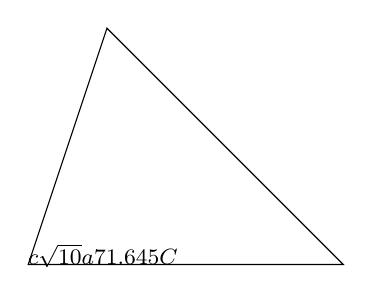
\begin{tikzpicture}[thin] \label{section-law-of-sin-and-cos-sinSAA}
					\coordinate (A) at (0,0);
					\coordinate (B) at (4,0);
					\coordinate (C) at (1,3);
					\draw (A)--(B)--(C)--cycle;
					\footnotesize
					\tkzLabelSegment[below=2pt](A,B){$c$}
					\tkzLabelSegment[above=2pt,rotate=atan(3)](A,C){$\sqrt{10}$}
					\tkzLabelSegment[above=2pt,rotate=-45](B,C){$a$}
					\tkzMarkAngle[size=1.1cm](B,A,C)
					\tkzLabelAngle[pos = 0.7](B,A,C){$\ang{71.6}$}
					\tkzMarkAngle[size=1cm](C,B,A)
					\tkzLabelAngle[pos = .7](C,B,A){$\ang{45}$}
					\tkzMarkAngle[size=.6cm](A,C,B)
					\tkzLabelAngle[pos = .4](A,C,B){$C$}
				\end{tikzpicture}
			\end{center}
		\end{multicols}
\end{myPractice}
\vfill

\begin{myPractice}
	\begin{multicols}{2}
		Use the law of sines to find the missing angles, $A$ and $C$, and the length, $a$, in the triangle in Figure \ref{section-law-of-sin-and-cos-sinSSA}. Round your answers to two digits behind the decimal place.
			\columnbreak
			\begin{center}\captionsetup{type=figure} \captionof{figure}{A triangle missing angles $A$ and $C$, and length $a$}
				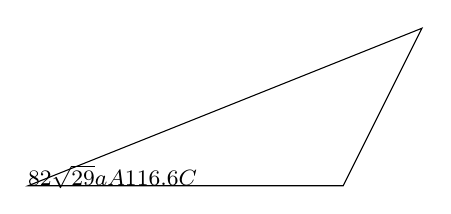
\begin{tikzpicture}[thin] \label{section-law-of-sin-and-cos-sinSSA}
					\coordinate (A) at (0,0);
					\coordinate (B) at (4,0);
					\coordinate (C) at (5,2);
					\draw (A)--(B)--(C)--cycle;
					\footnotesize
					\tkzLabelSegment[below=2pt](A,B){$8$}
					\tkzLabelSegment[above=2pt,rotate=atan(2/5)](A,C){$2\sqrt{29}$}
					\tkzLabelSegment[right=2pt](B,C){$a$}
					\tkzMarkAngle[size=1cm](B,A,C)
					\tkzLabelAngle[pos = 0.75](B,A,C){$A$}
					\tkzMarkAngle[size=0.9cm](C,B,A)
					\tkzLabelAngle[pos = .5](C,B,A){$\ang{116.6}$}
					\tkzMarkAngle[size=.7cm](A,C,B)
					\tkzLabelAngle[pos = .45](A,C,B){$C$}
				\end{tikzpicture}
			\end{center}
		\end{multicols}
\end{myPractice}
\vfill

%======================================================
\newpage
%======================================================

\begin{myPractice}
	\begin{multicols}{2}
		Use the law of cosines to find the missing angles, $A$ and $C$, and the length, $b$, in the triangle in Figure \ref{section-law-of-sin-and-cos-cosSSA}. Round your answers to two digits behind the decimal place.
			\columnbreak
			\begin{center}\captionsetup{type=figure} \captionof{figure}{A triangle missing angles $A$ and $C$, and length $b$}
				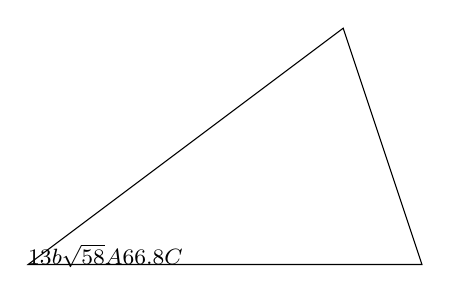
\begin{tikzpicture}[thin] \label{section-law-of-sin-and-cos-cosSSA}
					\coordinate (A) at (0,0);
					\coordinate (B) at (5,0);
					\coordinate (C) at (4,3);
					\draw (A)--(B)--(C)--cycle;
					\footnotesize
					\tkzLabelSegment[below=2pt](A,B){$13$}
					\tkzLabelSegment[above left=2pt](A,C){$b$}
					\tkzLabelSegment[above=2pt,rotate=-atan(7/3)](B,C){$\sqrt{58}$}
					\tkzMarkAngle[size=0.9cm](B,A,C)
					\tkzLabelAngle[pos = 0.6](B,A,C){$A$}
					\tkzMarkAngle[size=1.1cm](C,B,A)
					\tkzLabelAngle[pos = .7](C,B,A){$\ang{66.8}$}
					\tkzMarkAngle[size=.6cm](A,C,B)
					\tkzLabelAngle[pos = .35](A,C,B){$C$}
				\end{tikzpicture}
			\end{center}
		\end{multicols}
\end{myPractice}
\vfill

\begin{myPractice}
	\begin{multicols}{2}
		Use the law of cosines to find the missing angles, $A$, $B$, and $C$ in the triangle in Figure \ref{section-law-of-sin-and-cos-cosSSS}. Round your answers to two digits behind the decimal place.
			\columnbreak
			\begin{center}\captionsetup{type=figure} \captionof{figure}{A triangle missing angles $A$, $B$, and $C$}
				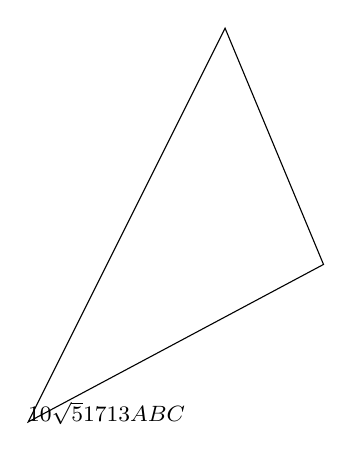
\begin{tikzpicture}[thin] \label{section-law-of-sin-and-cos-cosSSS}
					\coordinate (C) at (0,0);
					\coordinate (B) at (3.75,2);
					\coordinate (A) at (2.5,5);
					\draw (C)--(A)--(B)--cycle;
					\footnotesize
					\tkzLabelSegment[above=2pt,rotate=63](C,A){$10\sqrt{5}$}
					\tkzLabelSegment[below=2pt,rotate=28](C,B){$17$}
					\tkzLabelSegment[above=2pt,rotate=-67](A,B){$13$}
					\tkzMarkAngle[size=0.8cm](C,A,B)
					\tkzLabelAngle[pos = 0.5](C,A,B){$A$}
					\tkzMarkAngle[size=0.7cm](A,B,C)
					\tkzLabelAngle[pos = -.4](A,B,C){$B$}
					\tkzMarkAngle[size=1cm](B,C,A)
					\tkzLabelAngle[pos = .7](B,C,A){$C$}
				\end{tikzpicture}
			\end{center}
		\end{multicols}
\end{myPractice}
\vfill

%======================================================
\newpage
%======================================================

\subsection*{Definitions} \label{definitions-section-law-of-sin-and-cos}

\begin{myDefinition}[{Law of Sines}]~\\[0.5mm]
	The \textbf{law of sines} says that the ratios of sines of angles in a triangle and the opposite sides are all constant. That's a bit of a mouthful, maybe a math-ful will help. Consider the triangle in Figure \ref{section-law-of-sin-and-cos-definition-sines}. The law of sines says that...
	\[\frac{\sin(A)}{a}=\frac{\sin(B)}{b}=\frac{\sin(C)}{c}\text{\hspace{0.4cm} or alternately \hspace{0.4cm}}\frac{a}{\sin(A)}=\frac{b}{\sin(B)}=\frac{c}{\sin(C)}\]
\begin{center}\captionsetup{type=figure} \captionof{figure}{A triangle}
			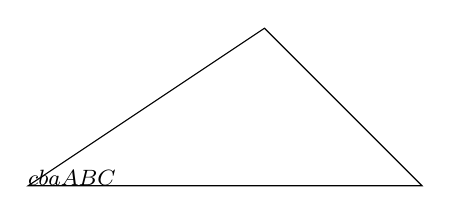
\begin{tikzpicture}[thin] \label{section-law-of-sin-and-cos-definition-sines}
				\coordinate (A) at (0,0);
				\coordinate (B) at (5,0);
				\coordinate (C) at (3,2);
				\draw (A)--(B)--(C)--cycle;
				\footnotesize
				\tkzLabelSegment[below=2pt](A,B){$c$}
				\tkzLabelSegment[above left=2pt](A,C){$b$}
				\tkzLabelSegment[above right=2pt](B,C){$a$}
				\tkzMarkAngle[size=0.9cm](B,A,C)
				\tkzLabelAngle[pos = 0.6](B,A,C){$A$}
				\tkzMarkAngle[size=0.8cm](C,B,A)
				\tkzLabelAngle[pos = .5](C,B,A){$B$}
				\tkzMarkAngle[size=.6cm](A,C,B)
				\tkzLabelAngle[pos = .35](A,C,B){$C$}
			\end{tikzpicture}
		\end{center}
		Note: When using the law of sines, you almost never need all three parts of the equation at the same time, so you will end up using one of these at a time:
		\[
			\frac{\sin(A)}{a}=\frac{\sin(B)}{b}\text{\hspace{0.4cm} or \hspace{0.4cm}}
			\frac{\sin(A)}{a}=\frac{\sin(C)}{c}\text{\hspace{0.4cm} or \hspace{0.4cm}}
			\frac{\sin(B)}{b}=\frac{\sin(C)}{c}
		\]
\end{myDefinition}
\vfill
\begin{myDefinition}[{Law of Cosines}]~\\[0.5mm]
	The \textbf{law of cosines} is really the natural extension of the Pythagorean Theorem for triangles without a right angle. Consider the triangle in Figure \ref{section-law-of-sin-and-cos-definition-cosines}. The law of cosines says that...
	\[a^2=b^2+c^2-2bc\cos(A)\text{\hspace{0.4cm} or \hspace{0.4cm}}b^2=a^2+c^2-2ac\cos(B)\text{\hspace{0.4cm} or \hspace{0.4cm}}c^2=a^2+b^2-2ab\cos(C)\]
		\begin{center}\captionsetup{type=figure} \captionof{figure}{A triangle}
			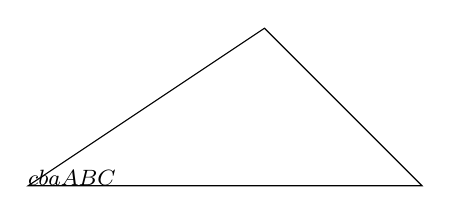
\begin{tikzpicture}[thin] \label{section-law-of-sin-and-cos-definition-cosines}
				\coordinate (A) at (0,0);
				\coordinate (B) at (5,0);
				\coordinate (C) at (3,2);
				\draw (A)--(B)--(C)--cycle;
				\footnotesize
				\tkzLabelSegment[below=2pt](A,B){$c$}
				\tkzLabelSegment[above left=2pt](A,C){$b$}
				\tkzLabelSegment[above right=2pt](B,C){$a$}
				\tkzMarkAngle[size=0.9cm](B,A,C)
				\tkzLabelAngle[pos = 0.6](B,A,C){$A$}
				\tkzMarkAngle[size=0.8cm](C,B,A)
				\tkzLabelAngle[pos = .5](C,B,A){$B$}
				\tkzMarkAngle[size=.6cm](A,C,B)
				\tkzLabelAngle[pos = .35](A,C,B){$C$}
			\end{tikzpicture}
		\end{center}
		Note: Unlike the Pythagorean Theorem, you \emph{don't} have to put the longest length alone on one side. It can be inputted for $a$, $b$, or $c$.
\end{myDefinition}
\vfill
%======================================================
\newpage
%======================================================

\subsection*{Exit Exercises} \label{exit-exercises-section-law-of-sin-and-cos}

\begin{myExit}
	\begin{enumerate}
		\item Michel\'e correctly wrote down these two equations about a triangle from a homework question. %https://www.desmos.com/calculator/ahc2lyhns2
		\[b^2=74+16^2-2\cdot\sqrt{74}\cdot16\cos(\ang{54.5})\text{\hspace{0.5cm} and \hspace{0.5cm}}\frac{\sin(C)}{16}=\frac{\sin(\ang{32.5})}{\sqrt{74}}\] 
		Draw the triangle from the question that these equations would have been based on.
		\vfill
		\begin{multicols}{2}
			\item On a steep hillside somewhere in the Cascades of Oregon stands a tall Douglas Fir. The slope is from point $B$, at the base of the tree, to the point $P$. The top of the tree is at point $T$. Some hikers wanted to get an estimate of its height, so they took a few measurements. They measured an angle of $\ang{52}$ from the vertically growing tree to the hillside slope using their inclinometer on their phones. Then they measured out $115\text{ft}$ up the hillside to point $P$ and measured the angle from there to be $\ang{83}$ from the base of the tree to the top of the tree, as shown in Figure \ref{section-law-of-sin-and-cos-DougFir}. Use the laws of sines or cosines to find an estimate for the height of the tree and round your answer to the nearest foot.
			\columnbreak
			\begin{center}\captionsetup{type=figure} \captionof{figure}{A Diagram of the Tree}
				\begin{tikzpicture}[thin] \label{section-law-of-sin-and-cos-DougFir}
					\begin{axis}[
						height=9cm,
						axis x line=none,
						axis y line=none,
						% xlabel=$x$,
						% ylabel=$y$,
						xlabel=none,
						ylabel=none,
						xmin=-10,xmax=110,
						ymin=-10,ymax=230,
						clip=false,
						]
							\node   [inner sep=0pt] (Doug Fir) at (1,110) {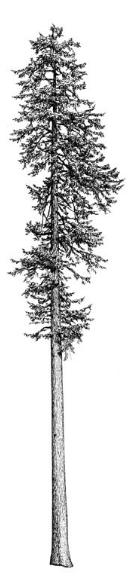
\includegraphics[width=.092\textwidth,angle=-1]{DougFir.png}};
							\draw   [thin,color=second](0,220) coordinate[label=above:$T$]--(90,70) coordinate[label=right:$P$]--(0,0) coordinate[label=below:$B$]--cycle;
        					\addplot[variable=\t, domain=30:90, samples=50,thin, color=third]({22*cos(t)}, {30*sin(t)});
        					\draw   (1,15)coordinate[label=right:\footnotesize$\ang{52}$];
        					\addplot[variable=\t, domain=127:210, samples=50,thin, color=third]({22*cos(t)+90}, {30*sin(t)+70});
        					\draw   (87,72)coordinate[label=left:\footnotesize$\ang{83}$];
        					\draw   (45,35)coordinate[label=below right:$115\text{ft}$];
					\end{axis}
				\end{tikzpicture}
			\end{center}
		\end{multicols}
		\vfill

		%======================================================
		\newpage
		%======================================================

		\item Imagine a triangle with sides $a=15$, $c=8$, and the angle $C=\ang{20}$, and length $b$, and angles $A$ and $B$ are unknown.
			\begin{enumerate}
				\item There are actually \emph{two} such triangles that exist. Draw pictures of both triangles.
				\vfill
				\item Write down the law of sines to solve for angle $A$ for each triangle, and compare the two equations.
				\vfill
				\item Solve for the angles and missing lengths in both triangles. Round your final answers for the angles and lengths to two digits behind the decimal place. \href{http://tiny.cc/ambiguous-triangles}{Check out this Desmos link} for a visual on these \say{ambiguous triangles}. \qrcode[height=1cm]{http://tiny.cc/ambiguous-triangles}
				\vfill
			\end{enumerate}
		\vfill
	\end{enumerate}
\end{myExit}
\exitlikert{the laws of sine and cosine}